\documentclass[
	11pt, 
	DIV10,
	a4paper, 
	oneside, 
	headings=normal, 
	captions=tableheading,
	final, 
	numbers=noenddot
]{scrartcl}


\usepackage{lipsum}
\usepackage{graphicx}
\usepackage[utf8]{inputenc}
\usepackage{subfigure}
\usepackage{amsmath}
\usepackage{float}
\usepackage{floatflt}
\usepackage{wrapfig}
\usepackage{csquotes}
\usepackage[multiple]{footmisc}

\title{Simulating Visual Geometry}
\subtitle{\vspace{0.5cm}Seminar: Current Topics in Physically-Based Animation}
\author{Patrick Bayer}


\begin{document}
\maketitle
\tableofcontents

\newpage

\section{Introduction}
	In this work, a new method for simulating deformation fracturing and tearing of visual geometry is introduced in order to get closer to the ultimate goal in virtual worlds namely "What you see is what you simulate". We want to provide a method which allows us to simulate objects in real time that are plastically and elastically deformable. These objects can even break or tear. Since the authors of the underlying paper do work on the PhysX Engine of nVidia this topic is essential for computer games and virtual reality, i.e. it directly bears upon the practice. Unfortunately it is easier said than done to achieve this goal because of performance restrictions in real time environments which is one reason for using multiple representation for rendering, simulating physical behaviour and collision detection. Also these objects are usually created with help of triangle or quad meshes that are well suitable for rendering or rigged kinematic animation but not for simulating physical behaviour.\\
	Therefore the new method uses a single representation for both, simulation and collision handling, and an almost identical representation for visualization whereas the simulation mesh is directly derived from the visual mesh. On the one hand the simulation mesh can be tuned independenty from the visual mesh and there are no restricitons on the structure of the input mesh but on the other hand creating such a simulation mesh can be problematic in case of gaps, overlapping of triangles or non-manifold vertices and edges. In addition to that we have to deal with possible visual artifacts such as a mismatch of collision behaviour and visual appearance. We also have to think of a solution for tearing and fracturing. \\
	Overall we want to take a short look on related papers because we use a few core ideas especially for the simulation method itself. We then take a closer look on the new method including the physical mesh creation, the simulation method, visualization and deformation of objects and in the end subdivision, fracturing and tearing. This work is based on the given paper \cite{1}. All the information that have no indication of source can be found in this paper. 
	
\section{Related Work}
	As already mentioned, a few core ideas form the basis of our simulation method. These ideas are using a general, non-conforming unstructured mesh, combining the rigid body formulation with a deformable model, fracture and tearing algorithms and a unified solver based on position based dynamics \cite{3}.

\subsection{Simulation Models}
	In order to create a proper simulation model people thought of plenty different ways to simulate objects. First mass-spring networks as in \cite{4} are used for hair simulation. Another early approach were regular grids in connection with finite differences \cite{5}. These have also been used in connection with finite elements resulting in the finite element method \cite{6}, the underlying method to simulate tetrahedal meshes which is the most popular representation for deformable volumetric objects. A further solution is to use the finite element method with help of the moving least square technique to simulate particles without connectivity as in \cite{7}. Last but not least we want to mention the material point method which is a hybrid method that has proven of value by using both particles and a grid \cite{8}, \cite{9} and \cite{10}.\\
	We will use the next approach, namely the oriented particle method \cite{2}, which is a generalization of the shape matching method and position based dynamics \cite{11}, to form the new method. A detailed explanation of how the method works is given in Section 3.\\
	Furthermore we use a unified solver based on position based dynamics. Since the original approach deals with sphere shaped particles and a position based rigid body formulation we need to extend it by adding the handling of convex polyhedra as primitives to simulate flat surfaces and sharp corners and edges. Bouaziz et al. also managed to reduce damping and to include the implicit Euler integration by adding an inertia term.\cite{12} Another way to achieve these results is to use a second order velocity update as introduced in \cite{3}.
	
\subsection{Embedding of a Visual Mesh}
	Because of the lack of quality, triangle or quad meshes can mostly be used for visualization but not to simulate physical behaviour. Sedeberg et al. came up with a fundamental idea by embedding the visual mesh in a simulation mesh.\cite{13} In this approach, objects are deformed by deforming a surrounding cage. Another approach introduced by Müller et al. describes a method where a visual mesh is embedded in a tretrahedal mesh \cite{14} and a regular grid \cite{6}. Moreover they describe how to deal with a fracture of the simulation mesh so that the mesh structure remains hidden and only the tear lines become visible.
	
\subsection{Fracturing and Tearing}
	The foundation for fracturing and tearing was laid by Terzopoulos et al. in \cite{5}. In their paper they use a given threshold to decide whether a link in a regular grid finite difference model needs to be broken. However O'Brian et al. did work with a tetrahedal mesh and the finite element method in order to determine the fracture direction with help of the stresses' direction inside the material. Unfortunately we can not afford the costs of such a stress analysis so that we have to fall back to a less expensive approach. For that reason we replace the model with pre-fractured models, which is not the best approach aswell, because we lose sight of the actual impact location. A proper approach that works for us is to use pre-defined fracture patterns that are applied at the impact location in connection with the representation of objects and fracture patterns with convex decompositions.\cite{15}
	\newpage
\section{The Method}

\subsection{Physical Mesh Creation}
	We start with a given visual mesh with triangle and quad faces that represents the objects surface. These faces are allowed to intersect each other. Some physical properties can be derived automatically from the objects geometry and those that cannot are defined by the user. Physical parameters are for instance thickness or material type.\\
	We want to use convex shapes as primitives in order to model flat surfaces and sharp corners and edges. A missing certain accuracy may cause problems after fracture events especially when the pieces are in close proximity as in Figure~\ref{GlassFracture}. We obtain these primitives in the form of convex polyhedra by extruding each face along the negative normal by the user defined thickness as we can see in the first row of Figure~\ref{PhysicalMeshCreation_1}. In case of enclosed convex shapes in the visual mesh we do not need to extrude them but to directly transform them into single primitives as shown in the 2D example in Figure~\ref{PhysicalMeshCreation_2} where the faces on the left side form enclosed convex shapes and can be directly transformed whereas the faces on the right side need to be extruded.\\
	Moreover we want to know something about the connections between each pair of primitives while using a general graph. We therefore look at the rest state of the object and decide that two primitives are connected in the graph if they touch or overlap. Typically we have to deal with more than a single visual mesh. In order to simulate a object as a whole these meshes get physically connected just like the primitives meaning if parts overlap. \\
	To build objects that possibly consist of several meshes it is possible for the user to connect sub-meshes via joints. These joints are defined by boxes. Their location and extent are determined by their pose while their names define the type and the participating bodies. An example is given in Figure~\ref{Joints}. \\
	\footnotetext[1]{Quelle: \cite{1}}
	\begin{minipage}{0.5\textwidth}
		\begin{figure}[H]
			\centering
			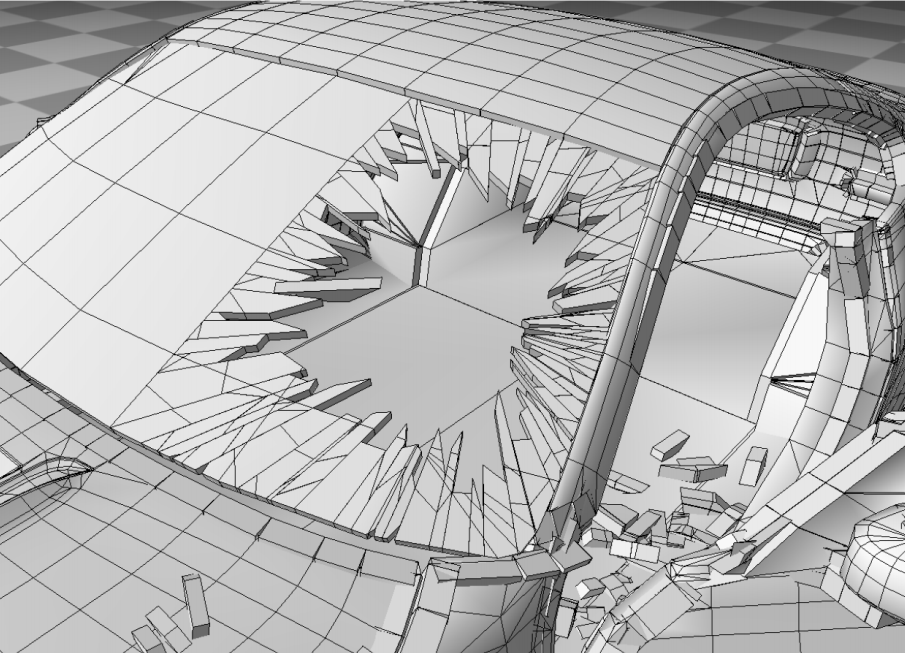
\includegraphics[scale = 0.26]{GlassFracture.PNG}
			\caption[caption]{\label{GlassFracture} \textit{A glass fracture pattern is applied to the car's window.}\footnotemark[1]}
		\end{figure}
	\end{minipage}
	\begin{minipage}{0.5\textwidth}
		\begin{figure}[H]
			\centering
			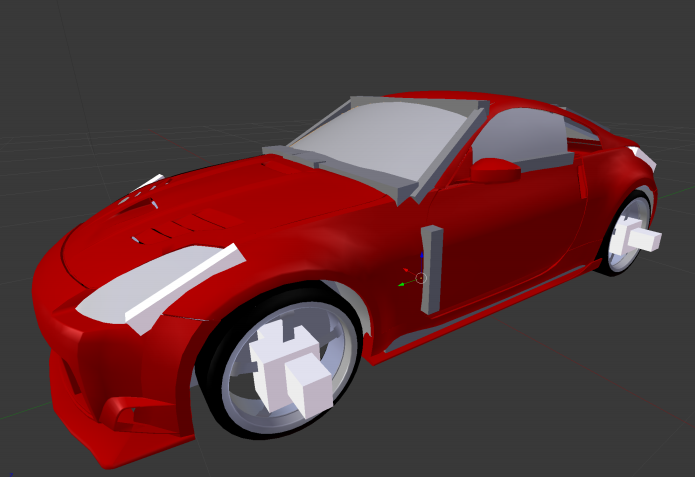
\includegraphics[scale = 0.34]{Joints.PNG}
			\caption[caption]{\label{Joints} \textit{Joint definition.} \footnotemark[1]}
		\end{figure}
	\end{minipage}
	\footnotetext[1]{Quelle: \cite{1}}
	\begin{minipage}{0.5\textwidth}
		\begin{figure}[H]
			\centering
			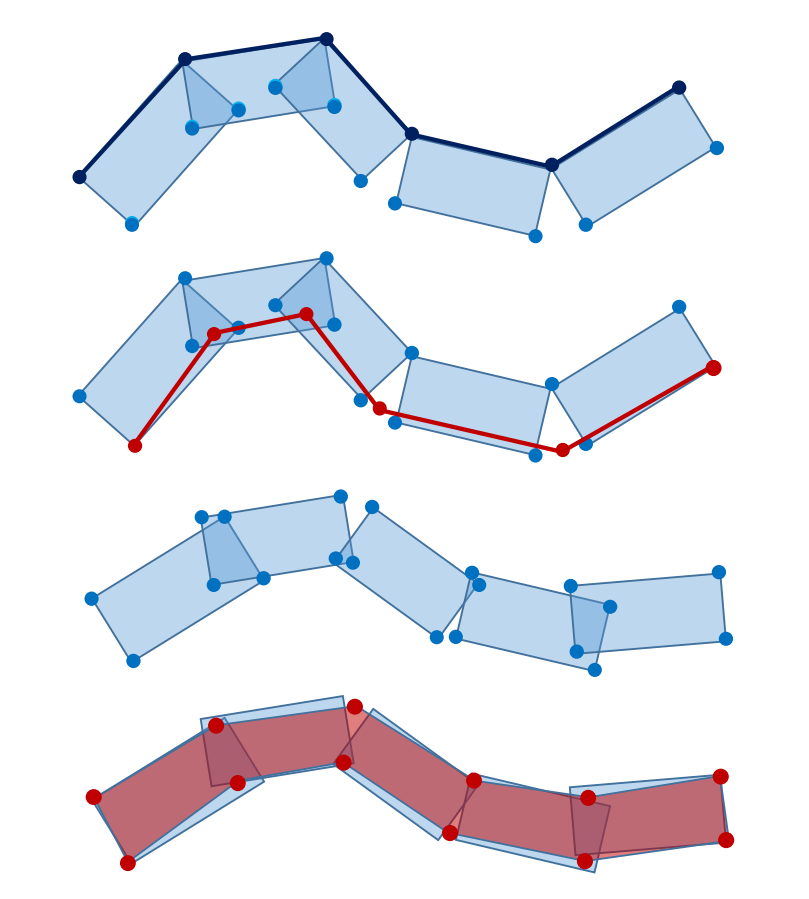
\includegraphics[scale = 0.27]{PhysicalMeshCreation_1.PNG}
			\caption[caption]{\label{PhysicalMeshCreation_1} \textit{From visual to simulation mesh(2d).}\footnotemark[1]}
		\end{figure}
	\end{minipage}
	\begin{minipage}{0.5\textwidth}
		\begin{figure}[H]
			\centering
			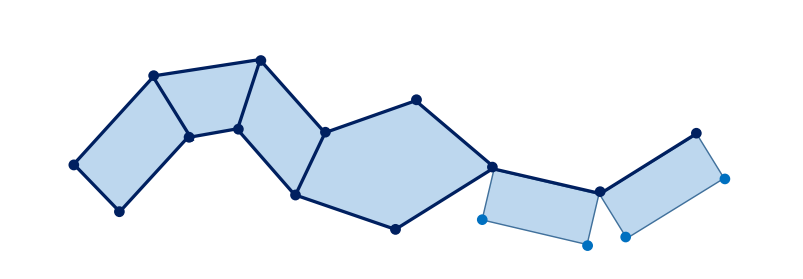
\includegraphics[scale = 0.3]{PhysicalMeshCreation_2.PNG}
			\caption[caption]{\label{PhysicalMeshCreation_2} \textit{Enclosed convex shapes are directly transformed into single primitives.}\footnotemark[1]}
		\end{figure}
	\end{minipage}

\subsection{The Simulation Method}
	The main idea is to use a unified solver that is able to handle convex polyhedra as primitives and the oriented particle method which is suitable for our simulation since the primitives have an orientation going hand in hand with their extent. Furthermore their connectivity defined as a general graph speaks in the methods favour. First we want to spend a few words on the oriented particle method itself. Usually the human eye can not see the difference between a hundred percent accurate simulation of physical behaviour of objects and a slightly worse one, especially when it comes to fast moving objects in games. On the other hand it is way more easy to notice a missing smoothness. Therefore the oriented particle method is simple aswell as fast. It uses particles that store their rotation and angular velocity next to the usual linear attributes such as position and velocity. In a few steps we will get to know the advantages from these additional information.\\  
	Unfortunately, in \cite{1} there is no explanation of how the method works so we want to take a closer look on generalized shape matching and position based dynamics.\\
	Before we get around to doing this we get ourselves introduced with collision handling whereat we can use the standard type based on sweep and prune for the broad phase and the seperate axis theorem for narrow phase because of using convex polyhedra. First we find intersections of the bounds of entire objects and identify all the cut-intersecting primitives. Next we identify the primitives that intersect each other and check carefully each individual pair of primitives for collision by using the seperating axis theorem. The seperating axis theorem essentially states if you are able to draw a line in 2D or a plane in 3D to seperate two primitives, they do not intersect.

\subsubsection{Generalized Shape Matching}
	Since the oriented particle method is a generalization of the shape matching method we want to get to know the foundation of the method. With shape matching we are able to model elasticity by pulling a deformed geometry towards a well-defined goal configuration. This method is stable and does not require any information of connectivity or specific representations because there is nothing but points.\cite{11}
	\footnotetext[1]{Quelle: \cite{11}}
	\begin{figure}[H]
		\centering
		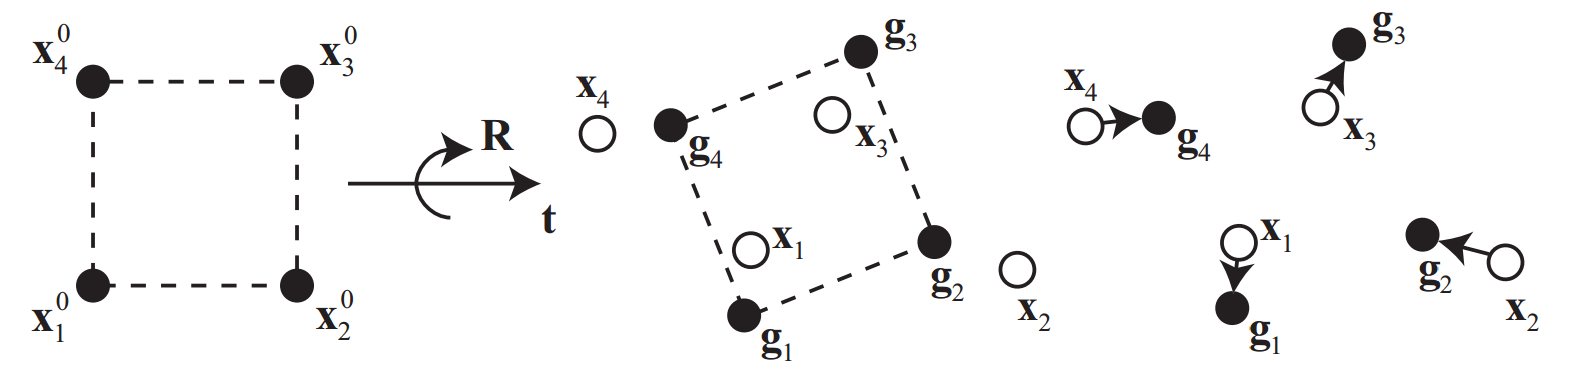
\includegraphics[scale = 0.36]{ShapeMatching.PNG}
		\caption[caption]{\label{ShapeMatching} \textit{Visualization of shape matching.}\footnotemark[1]}
	\end{figure}
	
	\noindent Figure~\ref{ShapeMatching} visualizes the functioning of the shape matching method. We start with a set of source points $\mathnormal{\mathbf{\bar{x}}_1,\dots,\mathbf{\bar{x}}_n}$ in their rest pose that store masses $\mathnormal{\mathbf{m}_i}$ with no connectivity or interaction between pairs of particles. In the end we want to find a goal configuration of our particle set. For that we need to compute a rotation matrix \textbf{R} and translation vectors \textbf{t} and $\mathnormal{\mathbf{\bar{t}}}$ applied on the initial configuration so that the distances between the goal positions $\mathnormal{\mathbf{g}_1,\dots,\mathbf{g}_n}$ and their corresponding current positions $\mathnormal{\mathbf{x}_1,\dots,\mathbf{x}_n}$ are minimized.\cite{11}
	For this purpose we need to solve the procrustes problem, i.e. to find $\mathbf{R}, \mathbf{\bar{t}}$ and $ \mathbf{t}$ to minimize
	\begin{center}
		$\sum\limits_{i}\mathnormal{\mathbf{m}_i}($\textbf{R}$(\mathnormal{\mathbf{\bar{x}}_i}-\mathnormal{\mathbf{\bar{t}}})+$\textbf{t}$-\mathnormal{\mathbf{x}_i})^2$
	\end{center}
	The optimal translation vectors turn out to be the center of mass of the initial configuration and the center of mass of the current configuration.\cite{11} We can compute them as follows.
	\begin{center}
		 $\mathnormal{\mathbf{\bar{t}}}=\mathnormal{\mathbf{\bar{x}}_{cm}}=\frac{\sum_{i}\mathnormal{\mathbf{m}_i} \mathnormal{\mathbf{\bar{x}}_i}}{\sum_{i}\mathnormal{\mathbf{m}_i}}$ and \textbf{t} $=\mathnormal{\mathbf{x}_{cm}}=\frac{\sum_{i}\mathnormal{\mathbf{m}_i \mathbf{x}_i}}{\sum_{i}\mathnormal{\mathbf{m}_i}}$
	\end{center}
	
	\noindent With help of these centers we determine the relative locations $\mathnormal{\mathbf{q}_i}=\mathnormal{\mathbf{\bar{x}}_i}-\mathnormal{\mathbf{\bar{x}}_{cm}}$ and\\
	$\mathnormal{\mathbf{p}_i}=\mathnormal{\mathbf{x}_i}-\mathnormal{\mathbf{x}_{cm}}$. Furthermore we want to relax the problem by searching an arbitrary matrix \textbf{A} instead of the optimal rotation matrix \textbf{R}. These changes lead to the following problem where we need to find $\mathbf{A}$ to minimize
	\begin{center}
		$\sum\limits_{i}\mathnormal{\mathbf{m}_i}(\mathnormal{\mathbf{A}\mathbf{q}_i}-\mathnormal{\mathbf{p}_i})^2$
	\end{center}
	\noindent After solving this minimization problem by setting the derivatives with respect to all coefficients of \textbf{A} to zero, the wanted matrix turns out to be
	\begin{center}
		\textbf{A} $=(\sum\limits_{i}\mathnormal{\mathbf{m}_i}\mathnormal{\mathbf{p}_i}\mathnormal{\mathbf{q}_i^T})(\sum\limits_{i}\mathnormal{\mathbf{m}_i}\mathnormal{\mathbf{q}_i}\mathnormal{\mathbf{q}_i^T})^{-1}=\mathnormal{\mathbf{A}}_{pq}\mathnormal{\mathbf{A}}_{qq}$
	\end{center}
	\noindent Since $\mathnormal{\mathbf{A}_{qq}}$ is symmetric it contains only scaling but no rotation, so the optimal rotation \textbf{R} is in the rotational part of $\mathnormal{\mathbf{A}_{pq}}$. A polar decomposition of $\mathnormal{\mathbf{A}_{pq}}$ yields
	\begin{center}
		$\mathnormal{\mathbf{A}_{pq}}=$ \textbf{RS} where \textbf{S} $=\sqrt{\mathnormal{\mathbf{A}_{pq}^T} \mathnormal{\mathbf{A}_{pq}}}$ and \textbf{R} $=\mathnormal{\mathbf{A}_{pq}}\mathnormal{\mathbf{S^{-1}}}$
	\end{center}
	\noindent Finally we computed all necessary parts to compute the goal positions $\mathnormal{\mathbf{g}_i}$ of each particle.
	\begin{center}
		$\mathnormal{\mathbf{g}_i}=\mathnormal{\mathbf{R}}(\mathnormal{\mathbf{\bar{x}}_i}-\mathnormal{\mathbf{\bar{x}}_{cm}})+\mathnormal{\mathbf{x}_{cm}}$ \cite{11}
	\end{center}

	\noindent Unfortunately this procedure becomes unstable when all points are (close to) co-planar or co-linear meaning that there exists a plane or a line that contains them all. In this case $\mathnormal{\mathbf{A}_{pq}}$ becomes ill-conditioned or singular yielding the optimal rotation matrix to not be well defined. The simulation gets unstable.\cite{2}\\
	At this point we profit from the orientation information of each particle because we want to achieve a well defined rotation \textbf{R} no matter what. First we introduce a reformulation of the definition of the moment matrix $\mathnormal{\mathbf{A}_{pq}}$ that will help us to compute a total moment matrix of the union of two particle sets with moment matrices $\mathnormal{\mathbf{A}_1}$ and $\mathnormal{\mathbf{A}_2}$. This matrix is defined as
	\begin{center}
		$\mathnormal{\mathbf{A}}=\sum\limits_{i}\mathnormal{\mathbf{m}_i \mathbf{x}_i \mathbf{\bar{x}}^T_i}-M\mathnormal{\mathbf{x}_{cm} \mathbf{\bar{x}}_{cm}^T}$
	\end{center}
	\noindent where $M$ is the sum of masses $\mathnormal{\mathbf{m}_i}$. Assuming that we can define such a moment matrix $\mathnormal{\mathbf{A}_i}$ for each particle \textit{i} we can shift the centers of masses to the center of mass of the particle set yielding
	\begin{center}
		$\mathnormal{\mathbf{A}}=\sum\limits_{i}(\mathnormal{\mathbf{A}_i}+\mathnormal{\mathbf{m}_i \mathbf{x}_i \mathbf{x}_i^T - \mathbf{m}_i \mathbf{x}_{cm} \mathbf{\bar{x}}_{cm}^T})$
	\end{center}
	In addition to that we can generalize the formulation of the matrix $\mathnormal{\mathbf{A}_{pq}}$ that gives us
	\begin{center}
		\begin{equation}\label{Apq}
			\mathnormal{\mathbf{A}_{pq}}=\sum\limits_{i}(\mathnormal{\mathbf{A}_i}+\mathnormal{\mathbf{m}_i \mathbf{x}_i \mathbf{\bar{x}}_i^T})-M\mathnormal{\mathbf{x}_{cm} \mathbf{\bar{x}}_{cm}^T}
		\end{equation}
	\end{center}
	
	\noindent Since we need the moment matrices with orthonormal orientation matrix \textbf{R} of single particles we have to integrate the equation over the particle's volume once for spheres with $V_r$ as the volume of radius $r$ and once for ellipsoids with radii $\mathnormal{a, b}$ and $\mathnormal{c}$ as follows.
	\begin{center}
		\begin{equation}\label{Asphere}
			\mathnormal{\mathbf{A}_{sphere}}= \int_{V_r}\rho(\mathbf{Rx})\mathbf{x}^T dV = \frac{1}{5}mr^2\mathbf{R}
		\end{equation}
	\end{center}
	\begin{center}
		$\mathnormal{\mathbf{A}_{ellipsoid}}= \frac{1}{5}m
		\begin{bmatrix}
			a^2& 0& 0 \\
			0& b^2& 0 \\
			0& 0& c^2
		\end{bmatrix}\mathbf{R}$
	\end{center} 
	\noindent With this extension we always get a full rank moment matrix \textbf{A} even for a single particle. \cite{2}
\subsubsection{Generalized Position Based Dynamics}
	Position based dynamics is an integration scheme that is used by the shape matching method. It basically works in three steps to simulate each particle which has a position $\mathbf{x}$ and a velocity $\mathbf{v}$. First we predict the position of each particle $\mathbf{x}_p$ using its velocity and the time step size $\mathbf{t}$ as follows.
	\begin{center}
		$\mathbf{x}_p \leftarrow \mathbf{x}+\mathbf{v}\Delta \mathbf{t}$
	\end{center}
	\noindent In the next step we want to correct the computed positions in order to satisfy several constraints by iterating through all constraints multiple times.\cite{2} Beside that we perform general shape matching and update both the velocity and the position of each particle yielding
	\begin{center}
		$\mathbf{v} \leftarrow \frac{\mathbf{x}_p - \mathbf{x}}{\Delta \mathbf{t}}$
	\end{center}
	\begin{center}
		$\mathbf{x} \leftarrow \mathbf{x}_p$
	\end{center}
	\noindent Stiffnes, friction and damping are handled as in regular PBD, i.e. they are defined as scalars.
	As already mentioned the primitives store additional information containing an orientation unit quaternion $\mathbf{q}$ and an angular velocity $\mathbf{\omega}$ that we want to update aswell during our simulation.
	For this purpose we extend the prediction and update step as follows.
	\begin{center}
		$\mathbf{q}_p \leftarrow [\frac{\mathbf{\omega}}{\vert \mathbf{\omega \vert}} sin(\frac{\vert \omega \vert \Delta \mathbf{t}}{2}), cos(\frac{\vert \omega \vert \Delta \mathbf{t}}{2})]\mathbf{q}$
	\end{center}
	\begin{center}
		$\mathbf{q} \leftarrow \mathbf{q}_p$
	\end{center}
	\begin{center}
		$\omega \leftarrow \frac{axis(\mathbf{q}_p \mathbf{q}^{-1})*angle(\mathbf{q}_p \mathbf{q}^{-1})}{\Delta \mathbf{t}}$
	\end{center}
	\noindent To remain the stability of the method we set $\mathbf{q}_p$ directly to $\mathbf{q}$ and $\omega$ to zero if $\vert \omega \vert$ or $\vert angle(\mathbf{q}_p \mathbf{q}^{-1})\vert$ falls below a certain threshold $\varepsilon$.\cite{2}
	
\subsubsection{Simulation Model}
	We define one shape matching group per particle which contains the corresponding particle and all the particles that are directly connected to it. These are used for soft body simulations and plasticity simulations inside rigid objects. Then the positions of the particles are computed and updated using the shape matching constraints that are previously introduced whereas only the orientation of the center particle is updated by replacing it with the optimal rotation. In this case we profit from our generalization of shape matching since it influences the orientation of the particle only along the directions contained in its moment matrix.\cite{2} In that way it will return the orientation of the only particle if there is only one. Otherwise it will return an orientation that is dominated by the orientation of the entire group. Shape matching is also used for stretching and bending provided that the artist does not want to specify them seperately. In this case we can use regular position based dynamics constraints.

\subsection{Deforming Primitives}
	Amongst others we pursue the goal of a visualization without any visual artifacts. This idea is not easy to fullfill since the oriented particle method only modifies the location and orientation of primitives. In that way potential gaps and collision artifacts can occur as we can see in Figure~\ref{PhysicalMeshCreation_1} and Figure~\ref{Curtain}. To avoid such visual artifacts we can not simply change the shapes of the primitives at will because we could destroy their property of being convex. We can not get away with that since that property is essential for collision handling and fracture. Instead we will use the local affine deformation matrix $\mathnormal{\mathbf{A}_{pq}}$ from Equation~\ref{Apq} where $\mathnormal{\mathbf{A}_i}$ are the moment matrices of each particle introduced in Equation~\ref{Asphere}.
	A generalization of the normalization of \cite{11} gives us the desired deformation matrix \textbf{D} that corresponds to the true best fit affine transformation.
	\begin{center}
		$\mathnormal{\mathbf{D}}=\mathnormal{\mathbf{A \bar{A}^{-1}}}$
	\end{center} 
	\noindent where
	\begin{center}
		$\mathbf{\bar{A}}=\sum\limits_{i}(\mathnormal{\mathbf{\bar{A}}_i+\mathbf{m}_i\mathbf{\bar{x}}_i\mathbf{\bar{x}}_i^T})-M\mathnormal{\mathbf{\bar{x}}_{cm} \mathbf{\bar{x}}_{cm}^T}$
	\end{center}
\noindent and $\mathnormal{\mathbf{A}_{i}}=\frac{1}{5}mr^2\mathbf{I}$.

\subsection{The Visualization Mesh}	
	As we can see in Figure~\ref{Curtain}, there are still visual gaps after deforming the primitives. In order to fix this problem, we use a visualization mesh that goes hand in hand with the simulation mesh and that grants us to use some of its attributes with fracturing and tearing in mind. Instead of attaching a general mesh to our simulation mesh we join the vertices of the primitives with respect to their positions. For this purpose each vertex gets an global identifier \textit{id}. Next we compute for each \textit{id} the average position of vertices with the same \textit{id} and store this information in an array with entries for each \textit{id}. Last but not least the vertices read back their position from the corresponding entry. In this way multiple vertices get the same identifier \textit{id}. A visualziation of this process is shown in Figure~\ref{PhysicalMeshCreation_1}. Here, the vertices are grouped and their positions are averaged in the second step. This yields a consistent inner surface in the rest state. After the third step, where the primitives change their poses during the simulation, the yielded gaps are closed using the averaged positions.
	\begin{wrapfigure}{R}{0.45\textwidth}
		\centering
		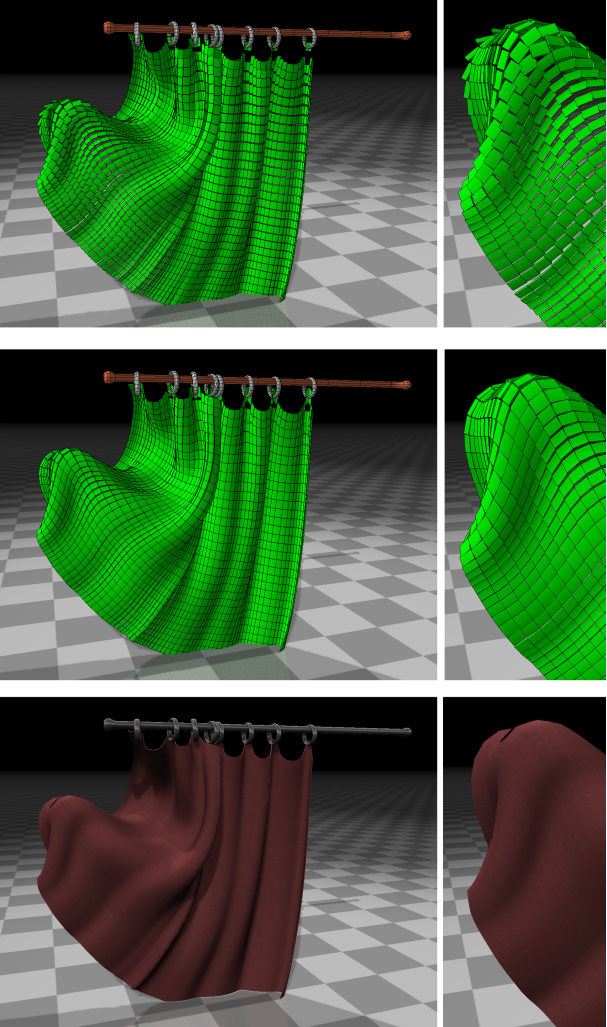
\includegraphics[scale = 0.34]{Curtain.PNG}
		\caption[caption]{\label{Curtain} \textit{Simulating a curtain using the oriented particle method and the local affine transformation of shape matching.} \footnotemark[1]}
	\end{wrapfigure}

\subsection{Plastic Deformation}
	To speed up our simulation we treat objects with rigid bodies as one rigid body until the primitives are plastically deformed and locally rearranged with the oriented particle method without harming the accuracy of our simulation since we are still using a detailed mesh for collision handling. Still we know nothing about when an object needs to be plastically deformed. Therefore we define a threshold for the relative normal velocity at each collision provided by the collision engine and check whether it is exceeded. We then compute the deformation offset as the relative normal velocity multiplied with the time step in order to displace the primitives. During further simulation the primitives that intersect the shapes of joints after deformation are considered fixed. At this point we can see how important it is to define joints with spatial extents because they serve as boundary conditions for our solver. Due to the fact that we change the local positions of the primitives the center of masses and inertia tensor change aswell and need to be re-computed.
	\footnotetext[1]{Quelle: \cite{1}}
\subsection{Subdivision, Fracturing and Tearing}
	Last but not least we want to take a look at how our method deals with subdivision, fracturing and tearing. At this point we profit again from using convex polyhedras as primitives because we can use the approach of Müller et al. \cite{15}.\\
	Starting with fracturing we introduce a connected set of convex polyhedra that acts as a fracture pattern that is aligned with the impact location. Next we find intersections of the bounds of the objects and the fracture pattern and compute all cut-intersecting primitives. This will result in new independent objects consisting of all pieces within a fracture cell. Since this approach just allows us to simulate brittle fracture, for instance used in Figure~\ref{GlassFracture}, we propose a modification that let us simulate ductile fracture aswell as adaptive level of detail. Instead of seperating the new objects immediatly after aligning the fracture pattern we keep them as one object in order to allow the simulation of details in regions with coarse meshes by forming detailed deformation patterns because a mesh is now subdivided close to an impact location. An example for details within coarse structurs is the deformation of the metal door in Figure~\ref{Door}.\\
	Along with this modification we propose two further extensions for ductile fracture and tearing. First we decide whether a connection between two primitives is broken by using a threshold for the distance between these primitives. We also do not want to be able to break all connections between the primitives because in this way the initial tesselation becomes visible where the fracture event occured. Furthermore the artist gets more control because he can pre-define tear lines by making only a subset of the connections breakable. Of course we do not only want subdivision, fracture and tearing to affect our simulation mesh but to become noticeable in visualization aswell. An easy way for this is to apply the fracture pattern in the undeformed configuration. In this way the old aswell as the new vertices that should be grouped can be identified as the ones that have the same positions. \\
	To continue with tearing we fall back on the identifier \textit{ids} of the primitives introduced in section 3.4 having in mind that primitives are connected if they share a common global \textit{id}. After we computed the number \textit{val(id)} of vertices that share each global \textit{id}, we can start with the actual tearing. Therefore we flood the graph which handles the connections between primitives by starting with a given primitive. However we just consider neighbours of our given primitive that share its global \textit{id}. If the number of visited vertices is smaller than \textit{val(id)}, a tear has occured. We then give the visited vertices a new \textit{id} and seperate them from the vertices that were not visited in the graph. Figure~\ref{Fracture} and Figure~\ref{Tearing} visualize the process of fracturing and tearing.\\
	At the end we need to update the joints by creating new joints with the same attributes for each from a fracture or tearing event resulting object that intersects the volume of the old joint. The old joints will no longer be needed and get deleted.
	\footnotetext[1]{Quelle: \cite{1}}
	\begin{figure}[H]
		\centering
		\subfigure{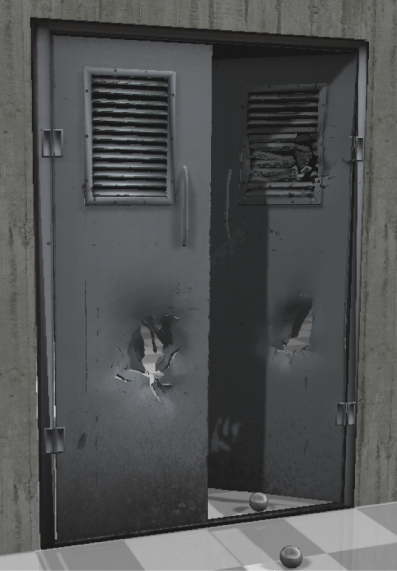
\includegraphics[scale = 0.35]{Door.PNG}}
		\subfigure{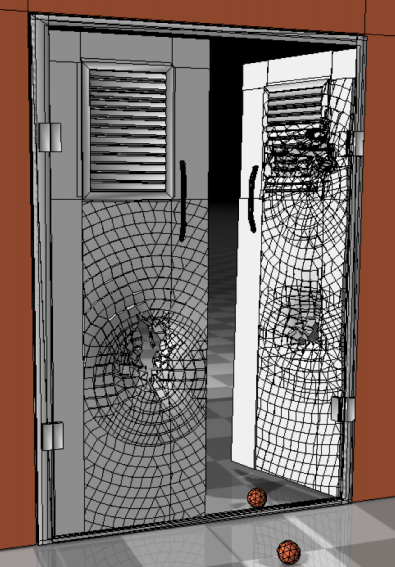
\includegraphics[scale = 0.35]{Door1.PNG}}
		\caption[caption]{\label{Door} \textit{Adaptive level of detail when deforming and tearing a metal door.} \footnotemark[1]}
	\end{figure}
	\begin{figure}[H]
		\centering
		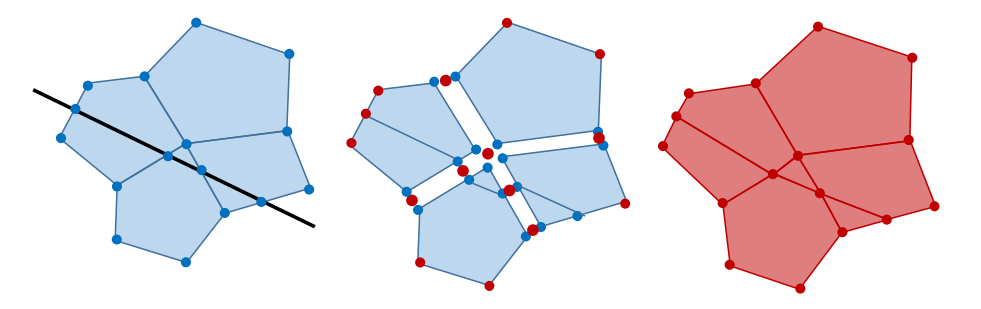
\includegraphics[scale = 0.4]{Fracture.PNG}
		\caption[caption]{\label{Fracture} \textit{Fracture of the visual mesh in the undeformed state.} \footnotemark[1]}
	\end{figure}

	\begin{figure}[H]
		\centering
		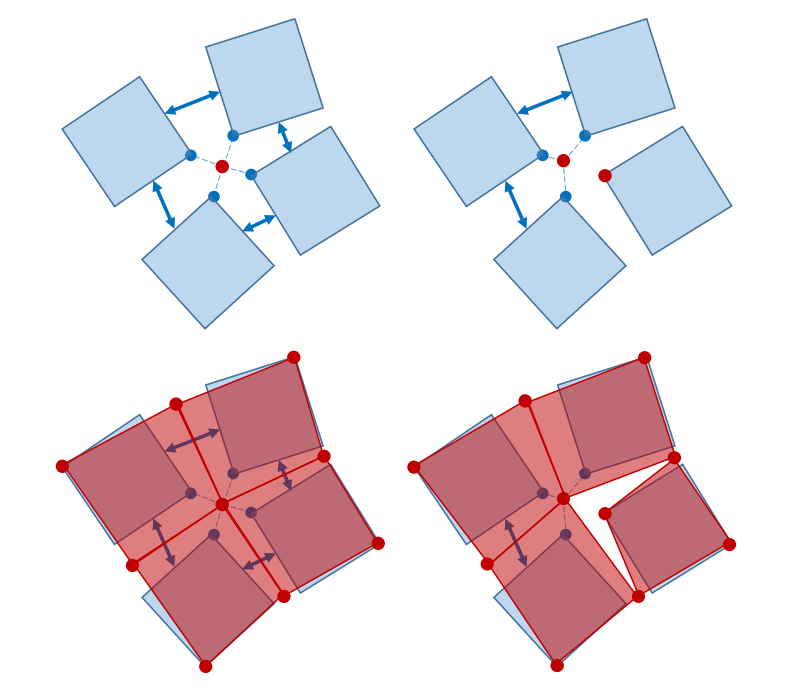
\includegraphics[scale = 0.38]{Tearing.PNG}
		\caption[caption]{\label{Tearing} \textit{Tearing of the visual mesh.} \footnotemark[1]}
	\end{figure}
	\footnotetext[1]{Quelle: \cite{1}}
\section{Conclusion}
	All in all a method was provided that is as fast and as simple as possible in order to get closer to the ultimate goal in virtual worlds namely "What you see is what you simulate". Therefore we introduced a physical mesh that can be directly derived from a given visual mesh with triangle and quad faces by using convex polyhedra as primitives and defining their connectivity. Using convex polyhedra as primitives speaks in many respects in favour of the oriented particle method so that we want to use this method for our simulation. Some of the results that are computed in the oriented particle method can also be used to improve the visualization meaning to remove visual gaps. Another advantage of convex polyhedra is that we can model flat surfaces and sharp corners and edges with tearing and fracture operations in mind. In addition to that standard collision algorithms work fine for this project.
	
\newpage

\begin{thebibliography}{15}
	\bibitem{1}Matthias Müller, Nuttapong Chentanez, Miles Macklin: Simulating Visual Geometry, Proceedings of the 9th International Conference on Motion in Games, 2016
	
	\bibitem{2}MÜLLER M., CHENTANEZ N.: Solid simulation with oriented
	particles. ACM Trans. Graph. 30, 4 (July 2011), 92:1–92:10
	
	\bibitem{3}BENDER J., MÜLLER M., MACKLIN M.: Position-based simulation
	methods in computer graphics. EUROGRAPHICS Tutorial
	Notes, Zürich, May 4-8 (2015)
	
	\bibitem{4}SELLE A., LENTINE M., FEDKIW R.: A mass spring model for
	hair simulation. ACM Trans. Graph. 27, 3 (Aug. 2008), 64:1–
	64:11
	
	\bibitem{5}TERZOPOULOS D., FLEISCHER K.: Modeling inelastic deformation:
	Viscoelasticity, plasticity, fracture. In the Proceedings of
	ACM SIGGRAPH 88 (1988), pp. 269–278
	
	\bibitem{6}MÜLLER M., TESCHNER M., GROSS M.: Physically-based simulation
	of objects represented by surface meshes. In in Proceedings
	of Computer Graphics International (CGI) (2004), pp. 26–
	33
	
	\bibitem{7}MÜLLER M., KEISER R., NEALEN A., PAULY M., GROSS M., ALEXA M.: Point Based Animation of Elastic, Plastic and Melting Objects. In Symposium on Computer Animation (2004), Boulic R., Pai D. K., (Eds.), The Eurographics Association
	
	\bibitem{8}STOMAKHIN A., SCHROEDER C., CHAI L., TERAN J., SELLE
	A.: A material point method for snow simulation. ACM Trans.
	Graph. 32, 4 (July 2013), 102:1–102:10
	
	\bibitem{9}STOMAKHIN A., SCHROEDER C., JIANG C., CHAI L., TERAN
	J., SELLE A.: Augmented mpm for phase-change and varied
	materials. ACM Trans. Graph. 33, 4 (July 2014), 138:1–138:11
	
	\bibitem{10}RAM D., GAST T., JIANG C., SCHROEDER C., STOMAKHIN
	A., TERAN J., KAVEHPOUR P.: A material point method
	for viscoelastic fluids, foams and sponges. In Proceedings of
	the 14th ACM SIGGRAPH / Eurographics Symposium on Computer
	Animation (2015), SCA ’15, pp. 157–163
	
	\bibitem{11}MÜLLER M., HEIDELBERGER B., TESCHNER M.: Meshless deformations
	based on shape matching. In Proc. SIGGRAPH 2005
	(2005), pp. 471–478
	
	\bibitem{12}BOUAZIZ S., MARTIN S., LIU T., KAVAN L., PAULY M.: Projective
	dynamics: Fusing constraint projections for fast simulation.
	ACM Trans. Graph. 33, 4 (July 2014), 154:1–154:11
	
	\bibitem{13}SEDERBERG T. W., PARRY S. R.: Free-form deformation of
	solid geometric models. In Proceedings of the 13th Annual
	Conference on Computer Graphics and Interactive Techniques
	(1986), SIGGRAPH ’86, pp. 151–160.
	
	\bibitem{14}MÜLLER M., GROSS M. H.: Interactive virtual materials. In
	Graphics Interface 2004 (London, Ontario, Canada, 2004),
	pp. 239–246.
	
	\bibitem{15}MÜLLER M., CHENTANEZ N., KIM T.-Y.: Real time dynamic
	fracture with volumetric approximate convex decompositions.
	ACM Trans. Graph. 32, 4 (July 2013), 115:1–115:10
\end{thebibliography}

\end{document}          
